\documentclass[12pt,letterpaper]{article}
\usepackage{fullpage}
\usepackage[top=2cm, bottom=4.5cm, left=2.5cm, right=2.5cm]{geometry}
\usepackage{amsmath,amsthm,amsfonts,amssymb,amscd}
\usepackage{lastpage}
\usepackage{enumerate}
\usepackage{fancyhdr}
\usepackage{mathrsfs}
\usepackage{xcolor}
\usepackage{graphicx}
\usepackage{listings}
\usepackage{hyperref}
\usepackage{amsmath}
\usepackage{mathtools}
\usepackage{tikz}
\usepackage{array}
\usetikzlibrary{matrix}

\hypersetup{%
  colorlinks=true,
  linkcolor=blue,
  linkbordercolor={0 0 1}
}
 
\renewcommand\lstlistingname{Section}
\renewcommand\lstlistlistingname{Algorithms}
\def\lstlistingautorefname{Alg.}

\lstdefinestyle{Python}{
    language        = Python,
    frame           = lines, 
    basicstyle      = \footnotesize,
    keywordstyle    = \color{blue},
    stringstyle     = \color{green},
    commentstyle    = \color{red}\ttfamily
}

\setlength{\parindent}{0.0in}
\setlength{\parskip}{0.05in}

% Edit these as appropriate
\newcommand\course{CSE 3500}
\newcommand\hwnumber{4}                  % <-- homework number
\newcommand\NetIDa{rjf23002}           % <-- NetID of person #1
\newcommand\NetIDb{}           % <-- NetID of person #2 (Comment this line out for problem sets)

\pagestyle{fancyplain}
\headheight 35pt
\lhead{\NetIDa}
\lhead{\NetIDa\\\NetIDb}                 % <-- Comment this line out for problem sets (make sure you are person #1)
\chead{\textbf{\Large Homework \hwnumber}}
\rhead{\course \\ \today}
\lfoot{}
\cfoot{}
\rfoot{\small\thepage}
\headsep 1.5em

\begin{document}

\section*{Problem 0}

\begin{enumerate}
  \item
    Suffix tree for BANDANNA (Blue) and SAVANNAH (Purple).
    \begin{figure}[!h]
      \centering
      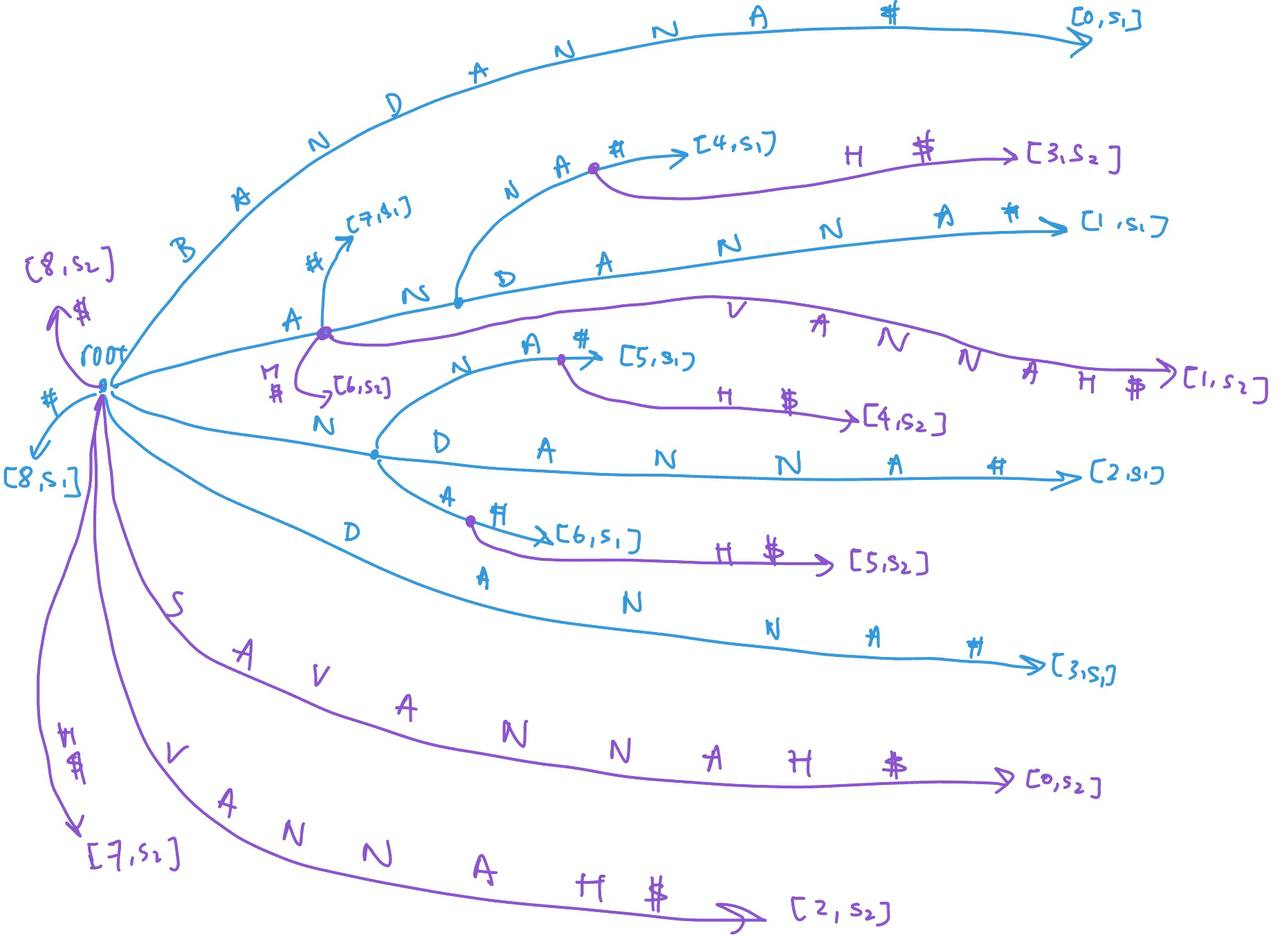
\includegraphics[width=1\linewidth]{suffixtree.jpg}
    \end{figure}
  \item
    We assume that the suffix tree has already been built before executing the algorithm.
    To find the longest common substring among m substrings,
    we can run a Depth First Search (DFS) algorithm.
    We are essentially looking for a node where the tree branches out into m different paths (each path must belong to each of the m substrings),
    such that the length of the suffix up till the branch is the longest.
    By looking for a node where the tree branches out into m paths, 
    this means that the suffix up till the branch exists as a suffix in all m strings.
    By performing DFS on the graph, we will also get to explore the entire graph,
    and will return the maximum length substring.
  \item 
    We will have to explore the whole graph.
    The size of our graph is bounded by the number of nodes which is in turn
    bounded by the length of each string.
    We let the length of each string be $n_{1}, n_{2}, ..., n_{m}$.
    Thus, the total time complexity would be $\sum^{m}_{i=1} O(n_{i})$.
  \item 
    Using our algorithm, we can find the longest common substring to be 'ANNA'. \\
    This can be found by tracing down each root, where we eventually hit the path starting from 'A'.
    At 'A', we see that it does branch out into substring 1 (s1) and substring 2 (s2). 
    Thus, 'A' is indeed a valid substring.
    However, exploring the same path, we do see that another valid substring exists.
    We can see that 'ANNA' also branches out to s1 and s2. 
    Since it is longer, we can take it to be the maximum.
    We continuously perform this check on all paths, and will eventually find that 'ANNA' is the longest.
\end{enumerate}

\section*{Problem 1}

\begin{enumerate}
  \item
    Let us assume we want to find the longest palindromic substring in a string S.
    An approach to do so using suffix tree would be to combine another suffix tree S' on top of S.
    S' should be the suffix tree of the reversed string of S.
    By combining them, we can then use the LCS algorithm from Problem 0 to determine the longest palindromic substring among S and S'.
  \item 
    The time complexity to create suffix tree S and S' would be bounded by O(n).
    The time complexity to perform LCS on this tree would also be O(n) since both strings are of equal lengths.
    Thus, it is bounded by O(n).
  \item 
    Let S be 'RACECARS' and S' be 'SRACECAR'. 
    We form two suffix trees based of these strings.
    We perform the same LCS algorithm, realizing that there exists a longest path from R.
    It only splits out at RACECAR into two branches, one from string S and another from S'.
    Hence, the LCS algorithm returns us RACECAR as the longest common substring.
    Since, we are comparing a string S to its reversed form S', thus the longest palindromic substring is then RACECAR as well.
\end{enumerate}

\section*{Problem 2}

\begin{enumerate}
  \item
    Let us populate the suffix array with indexes for the string REPETITIVE such that the starting index of character 'R' is 0 and 'E' being 9 \\\\
    We have the following suffixes: \\
    REPETITIVE, index 0 \\
    EPETITIVE, index 1  \\
    PETITIVE, index 2  \\
    ETITIVE, index 3  \\
    TITIVE, index 4  \\
    ITIVE, index 5  \\
    TIVE, index 6  \\
    IVE, index 7 \\
    VE, index 8  \\
    E, index 9  \\\\
    Arranging the suffixes in lexicographical order, we have: \\
    E, index 9  \\
    EPETITIVE, index 1  \\
    ETITIVE, index 3  \\
    ITIVE, index 5  \\
    IVE, index 7 \\
    PETITIVE, index 2  \\
    REPETITIVE, index 0 \\
    TITIVE, index 4  \\
    TIVE, index 6  \\
    VE, index 8  \\

    Hence, the suffix array is given by: \\
    $[10, 9, 1, 3, 5, 7, 2, 0, 4, 6, 8]$
  \item
    To find occurrences of a string P in a larger string S, 
    we first construct the suffix array and LCP array.
    We can then do binary search to find the very first index in the LCP array which has the occurrence of P.
    We then iterate from left to right, where each iteration increases our result by 1. 
    We terminate by checking the LCP array until the count hits 0.
    As the LCP array is sorted lexicographical, when the count hits 0, 
    it means we have gone to a suffix starting with another word.
    Hence, there is no need to continuously check.
  \item 
    If we are looking for speed, then suffix tree should be the choice to go.
    This is because it has several optimizations such as links which may help speed up querying time.
    The trade off is that might incur a bit more space, as we have to implement a Node struct.
    If space is not a concern, suffix trees might be the better option.
\end{enumerate}

\section*{Problem 3}

Let us define a random variable X such that $X_{s}$ = 1 if h(a) = h(b) and 0 otherwise.
X is a rv equal to the number of elements s (a subset of S) for which h(a) = h(b).
For any pair of elements, u, v, the probability that a random chosen h (a subset of H) is at most 1/n by universality. 
Let X equal to the summation of $X_{s}$, such that we have $|S|$ * 1/n, 
where $|S|$ is the size of the output table, m. 
Hence, we need m/n elements.

\end{document}
